% Using Free and Open Source Solutions in Geospatial Science Education
% This work by Vaclav Petras is licensed under
% a Creative Commons Attribution-ShareAlike 4.0 International License.

\documentclass[xcolor={dvipsnames,usenames},beamer,aspectratio=169]{beamer}
% ,handout,notes=show

\makeatletter
\def\beamer@framenotesbegin{% at beginning of slide
  \gdef\beamer@noteitems{}%
  \gdef\beamer@notes{{}}% used to be totally empty.
}
\makeatother

\usepackage{textcomp}
\usepackage[utf8]{inputenc}
\usepackage[american]{babel}
\usepackage{graphicx}
\usepackage{url}
\usepackage{amssymb}

\usepackage{tikz}
\usetikzlibrary{arrows,shapes,spy,calc}

\tikzstyle{every picture}+=[remember picture]
\tikzstyle{na} = [baseline=-.5ex]

% frames have to be fragile
\newif\ifnotes
% \input{tmpnotessettings}
% \notestrue


\ifnotes
\setbeamertemplate{note page}[plain]
% \setbeamertemplate{note page}[compress]
\setbeamerfont{note page}{size=\large}
% \setbeameroption{show only notes}
\setbeameroption{show notes}
\usepackage{pgfpages}
\pgfpagesuselayout{2 on 1}[a4paper,border shrink=5mm]%
\else
%\setbeameroption{hide notes}
\fi
%\notesfalse

\usepackage[absolute,overlay]{textpos}

\usepackage{listings}


% \usetheme{Warsaw}
\usetheme{Madrid}
% \usetheme{Frankfurt}
% \useoutertheme{infolines}
\usecolortheme[named=MidnightBlue]{structure}
% \usecolortheme[named=PineGreen]{structure}
\setbeamertemplate{navigation symbols}{}

\setbeamertemplate{itemize items}[default]
\setbeamertemplate{enumerate items}[default]
% \useinnertheme{rectangles}
\setbeamertemplate{blocks}[default]


%%%%%%%%%%%%%%%%%%%%%%%%%%%%%%%%%%%%%%%%%%%%%%%%%%%%%%%%%%%%%%%%%%%%
%%%%%%%%%%%%%%%%%%%%%%%%%%%%%%%%%%%%%%%%%%%%%%%%%%%%%%%%%%%%%%%%%%%%

% \newcommand{\n}[1]{$^{\color{gray}{\mbox{\tiny#1}}}$}
\newcommand{\n}[1]{$^{\textcolor{gray}{\mbox{\tiny{#1}}}}$}

%%%%%%%%%%%%%%%%%%%%%%%%%%%%%%%%%%%%%%%%%%%%%%%%%%%%%%%%%%%%%%%%%%%%%%%%%%%%%%%
\newcommand{\gmodule}[1]{\href{http://grass.osgeo.org/grass71/manuals/#1.html}{\emph{#1}}}
\newcommand{\asixmodule}[1]{\emph{#1}}
\newcommand{\asevenmodule}[1]{\emph{#1}}
\newcommand{\module}[1]{\emph{#1}}
\newcommand{\grasslink}{\href{http://grass.osgeo.org/}{GRASS GIS}}

%%%%%%%%%%%%%%%%%%%%%%%%%%%%%%%%%%%%%%%%%%%%%%%%%%%%%%%%%%%%%%%%%%%%
%%%%%%%%%%%%%%%%%%%%%%%%%%%%%%%%%%%%%%%%%%%%%%%%%%%%%%%%%%%%%%%%%%%%

\title%[Processing of point clouds]
{New lidar processing functionality in GRASS GIS 7.1}
\subtitle{webinar for U.S. Fish and Wildlife Service Remote Sensing Technical Group}
%\pdforstring{}{}

\author[Vaclav Petras]
{Vaclav Petras (Vashek)%\n{1}\\
%{\scriptsize
%Anna Petrasova\n{1},
%\mbox{
%Helena Mitasova\n{1}
%}
%}
}

\institute[NC State University]
{%
%$^1$%
Center for Geospatial Analytics \\
\bigskip

\includegraphics[width=0.3\textwidth]{logos/ncstate}
}

\date{February 22, 2016}

\setbeamercovered{transparent}

\hypersetup{%
 pdfauthor={Vaclav Petras},%
 pdfsubject={UAV/lidar data analytics course project presentation},%
 pdfkeywords={UAV} {UAS} {point clouds} {lidar}
   {v.in.lidar} {r.in.lidar} {v.decimate} {v.out.lidar} {libLAS}
   {geospatial modeling} {GRASS GIS}
   {free software} {open source} {open science}
}

\usepackage{tipa}
\newcommand{\pron}[2]{#1 [#2]}


\newcommand{\beginbackup}{
  \newcounter{framenumbervorappendix}
  \setcounter{framenumbervorappendix}{\value{framenumber}}
}
\newcommand{\backupend}{
  \addtocounter{framenumbervorappendix}{-\value{framenumber}}
  \addtocounter{framenumber}{\value{framenumbervorappendix}}
}


%%%%%%%%%%%%%%%%%%%%%%%%%%%%%%%%%%%%%%%%%%%%%%%%%%%%%%%%%%%%%%%%%%%%
% when images are placed in these directories, we don't have to specify the directory
% just the filename
\graphicspath{{img/}{figures/}{images/}}


%%%%%%%%%%%%%%%%%%%%%%%%%%%%%%%%%%%%%%%%%%%%%%%%%%%%%%%%%%%%%%%%%%%%
%%%%%%%%%%%%%%%%%%%%%%%%%%%%%%%%%%%%%%%%%%%%%%%%%%%%%%%%%%%%%%%%%%%%
%%%%%%%%%%%%%%%%%%%%%%%%%%%%%%%%%%%%%%%%%%%%%%%%%%%%%%%%%%%%%%%%%%%%
%%%%%%%%%%%%%%%%%%%%%%%%%%%%%%%%%%%%%%%%%%%%%%%%%%%%%%%%%%%%%%%%%%%%
\begin{document}

\newcommand{\logowidth}{1.0em}
\newcommand{\logospace}{\hspace{0.2em}}
\newcommand{\includecclogo}[1]{\includegraphics[width=\logowidth]{./images/logos/#1}}

%%%%%%%%%%%%%%%%%%%%%%%%%%%%%%%%%%%%%%%%%%%%%%%%%%%%%%%%%%%%%%%%%%%%
\frame{
\titlepage
\begin{center}
\vspace{-3ex}
\href{http://creativecommons.org/licenses/by-sa/4.0/}{
\includecclogo{cc}
\logospace
\includecclogo{by}
\logospace
\includecclogo{sa}
}
\\
\footnotesize
available at\\
\href{http://wenzeslaus.github.io/grass-lidar-talks/}{\texttt{wenzeslaus.github.io/grass-lidar-talks}}
\end{center}
}


%%%%%%%%%%%%%%%%%%%%%%%%%%%%%%%%%%%%%%%%%%%%%%%%%%%%%%%%%%%%%%%%%%%%%
\begin{frame}{GRASS GIS}

\begin{columns}
\begin{column}{0.4\textwidth}

 \begin{itemize}
  \item functionality split to modules
  \item unified access to all modules from GUI, command line, Python and R
  \item GUI independent but integrated
  \item all in one
\end{itemize}

\begin{center}

\includegraphics[width=0.3\textwidth]{logos/grass_gis}
\end{center}

\end{column}
\begin{column}{0.55\textwidth}

\begin{center}
  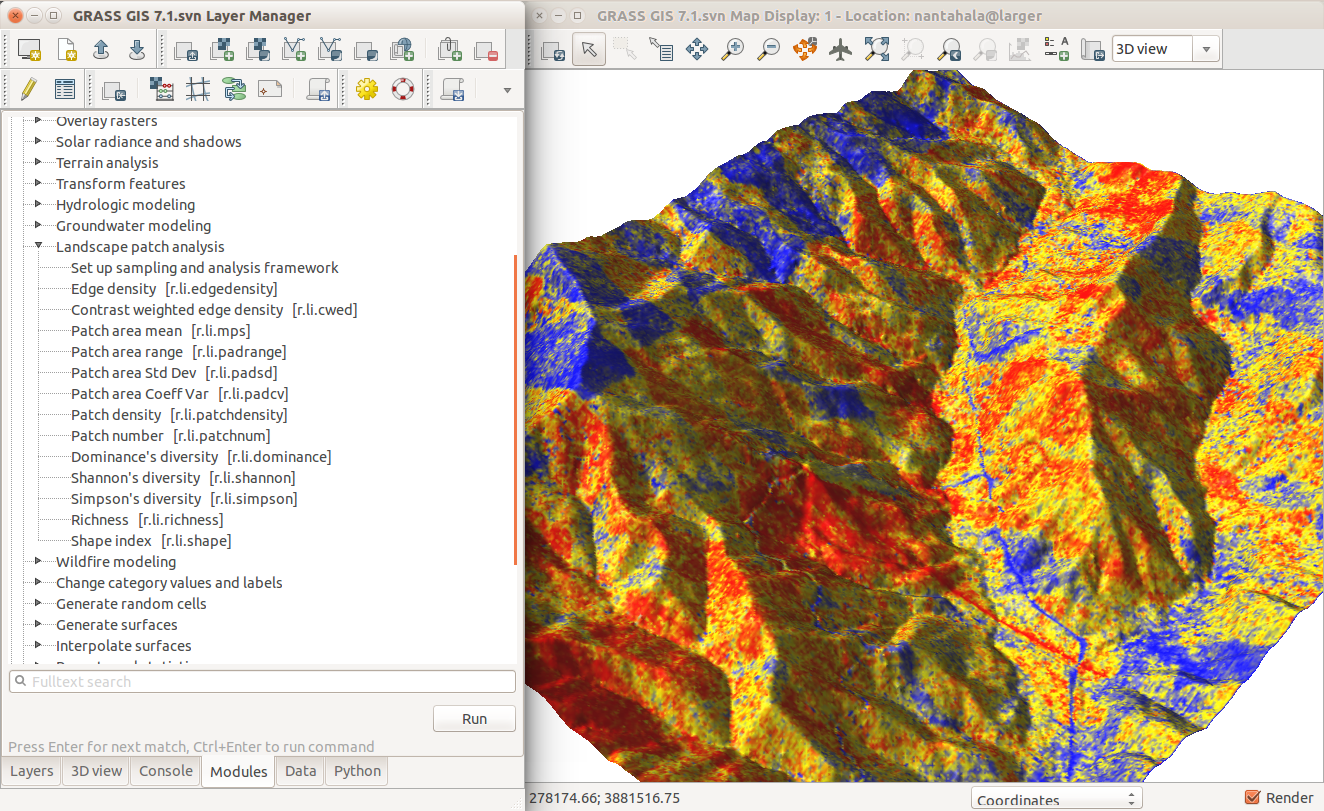
\includegraphics[width=\textwidth]{grass/count_and_modules}
\end{center}

\end{column}
\end{columns}

\end{frame}


%%%%%%%%%%%%%%%%%%%%%%%%%%%%%%%%%%%%%%%%%%%%%%%%%%%%%%%%%%%%%%%%%%%%%
\begin{frame}{Typical lidar workflow}

\begin{columns}
\begin{column}{0.5\textwidth}

% \begin{block}{Explore the data with \gmodule{r.in.lidar}}
Explore the data with \gmodule{r.in.lidar}
 \begin{itemize}
  \item import extent based on input data (\texttt{-e}~flag)
  \item resolution set to high number (coarse, \texttt{resolution=10})
  \item count number of points per cell (\texttt{method=n})
  \item try different class and return filters (\texttt{class\_filter}, \texttt{return\_filter})
  \item decide on computational region extent and resolution (\texttt{g.region})
 \end{itemize}
% \end{block}

\end{column}
\begin{column}{0.45\textwidth}

\begin{center}
  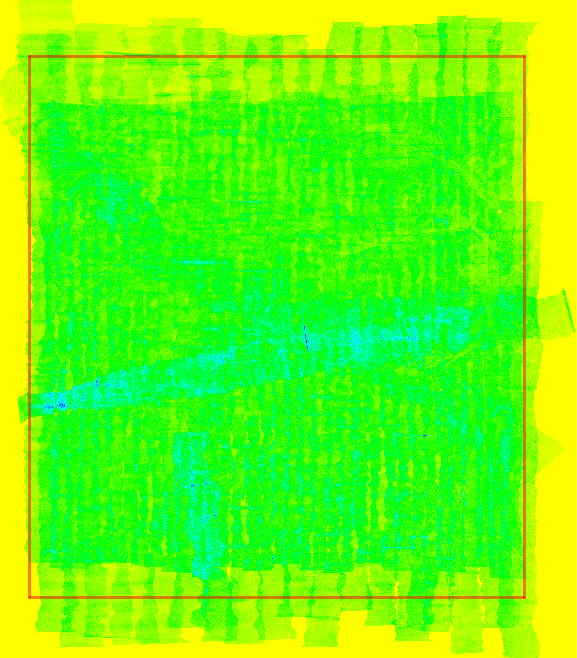
\includegraphics[width=0.75\textwidth]{grass/rinlidar_region}

  \footnotesize
  r.in.lidar, 578 million points in 90 files to 1882 $\times$ 1651 cells using 50MiB in 2 min

% time r.in.lidar file=list_las_files.txt -e method=n output=count res=5 --o
% 578628031 points from 90 files found in region
%
% r.in.lidar: 2m14.852s 50MiB
% r.info map=count@all -g
% north=3886000
% south=3876590
% east=281705
% west=273450
% nsres=5
% ewres=5
% rows=1882
% cols=1651
% cells=3107182
% datatype=CELL
% ncats=0
%
% r.in.lidar: 2m25.048s 1.2GiB
% r.info map=count_2@all -g
% north=3886000
% south=3876590.5
% east=281700.5
% west=273452
% nsres=0.5
% ewres=0.5
% rows=18819
% cols=16497
% cells=310457043
% datatype=CELL
% ncats=0

% g.region rast=count_2@all
% r.univar map=count_2@all -e
% 30 sec

\end{center}

\end{column}
\end{columns}

\end{frame}


%%%%%%%%%%%%%%%%%%%%%%%%%%%%%%%%%%%%%%%%%%%%%%%%%%%%%%%%%%%%%%%%%%%%%
\begin{frame}{Typical lidar workflow}


\begin{columns}
\begin{column}{0.5\textwidth}

Analyze with \gmodule{r.in.lidar}
 \begin{itemize}
  \item statistics of point counts, height and intensity
  \item using different resolutions
 \end{itemize}

Create surface with \gmodule{v.in.lidar} and interpolation
 \begin{itemize}
  \item few/sparse points, smaller extent
%   \item import selected points (spatial extent, classes and returns)
  \item interpolate smooth surface without NULLs
  \end{itemize}

Continue analysis using standard GRASS GIS tools
% rasterize soon (if you can)

\end{column}
\begin{column}{0.45\textwidth}

\begin{center}
  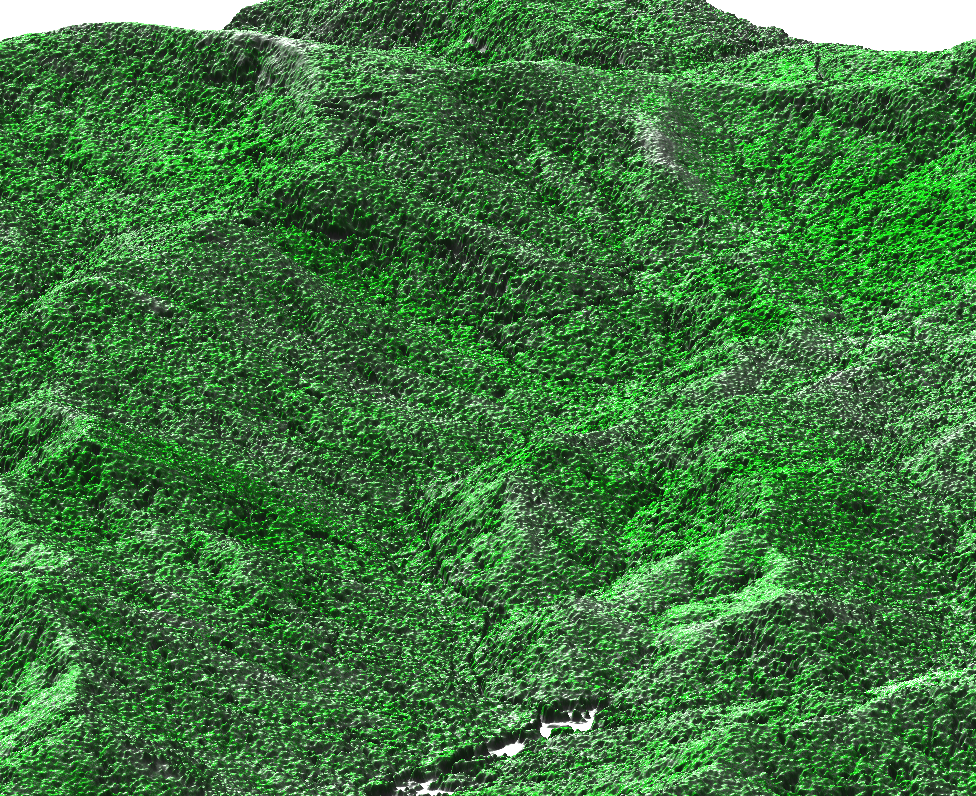
\includegraphics[width=0.8\textwidth]{grass/range_on_smooth_max_larger}

  \footnotesize
  r.in.lidar and r.neighbors, range smoothed maximum surface,
  551 million points from 90 files to 8076 x 7223 cells
  using 480MiB in 4 min
  % 1 + 37.262/60 + 1 + 47.132/60 + 11./60
\end{center}

% g.region -p
% north:      3885316.5
% south:      3877241.5
% west:       273832
% east:       281053
% nsres:      0.5
% ewres:      0.5
% rows:       16150
% cols:       14442
% cells:      233238300

% r.in.lidar max
% 550927433 points from 90 files found in region
% 920MiB
% 1m39.372s

% g.region -p
% north:      3885316.5
% south:      3877241.25
% west:       273831.75
% east:       281053.5
% nsres:      0.75
% ewres:      0.75
% rows:       10767
% cols:       9629
% cells:      103675443

% r.in.lidar max
% 550927433 points from 90 files found in region
% 430MiB
% 1m38.932s


% g.region -p
% north:      3885317
% south:      3877241
% west:       273831
% east:       281054
% nsres:      1
% ewres:      1
% rows:       8076
% cols:       7223
% cells:      58332948

% r.in.lidar max
% 550927433 points from 90 files found in region
% 250MiB
% 1m37.262s

% r.neighbors input=max size=7
% 11 sec

% r.in.lidar range
% 550927433 points from 90 files found in region
% 480MiB
% 1m47.132s

% r.in.lidar skewness
% 551004149 points from 90 files found in region
% 8.5 GiB
% 3m10.144s

% r.in.lidar mean class=2
% 28,669,253 points from 90 files found in region
% 480MiB
% 2 min 10 sec

% r.neighbors -c --overwrite input=ground_mean size=25
% 2 min 33 sec

\end{column}
\end{columns}

\end{frame}


%%%%%%%%%%%%%%%%%%%%%%%%%%%%%%%%%%%%%%%%%%%%%%%%%%%%%%%%%%%%%%%%%%%%%
\begin{frame}{UAV/lidar Data Analytics course at NCSU}

\begin{itemize}
  \item openly (and freely) accessible study materials
  \item GRASS GIS, Python, Agisoft Photoscan (proprietary), OpenDroneMap
  \item \url{http://ncsu-osgeorel.github.io/uav-lidar-analytics-course/}
\end{itemize}

\centering
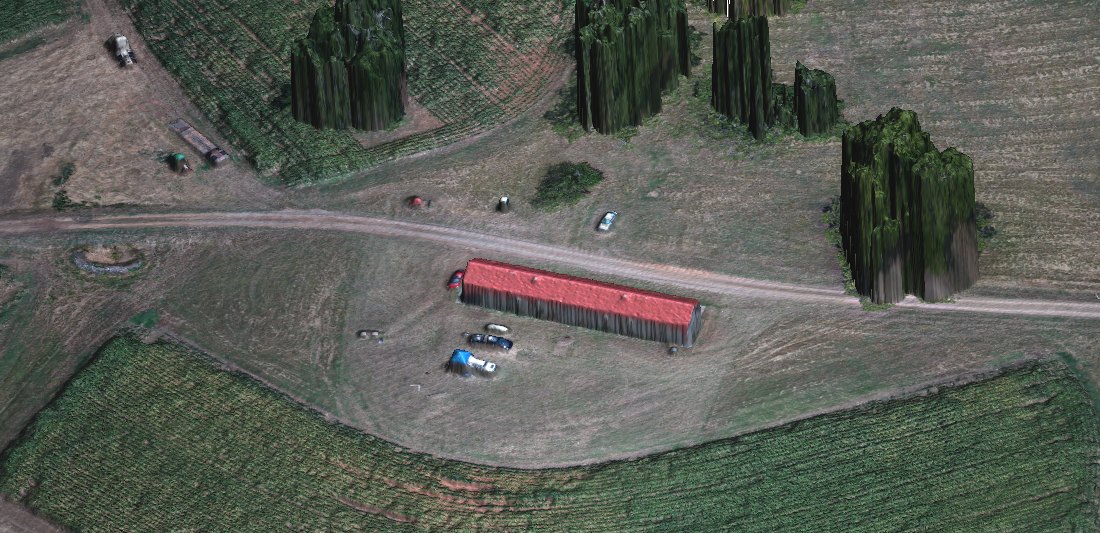
\includegraphics[width=0.7\textwidth]{agisoft_detail}%

\end{frame}

%%%%%%%%%%%%%%%%%%%%%%%%%%%%%%%%%%%%%%%%%%%%%%%%%%%%%%%%%%%%%%%%%%%%%
\begin{frame}{r.in.lidar}

\begin{columns}
\begin{column}{0.4\textwidth}


\begin{itemize}
  \item one file or multiple files as input
  \item produces raster from points
  \begin{itemize}
    \item n, min, max, range
    \item sum, mean, skewness, \ldots
  \end{itemize}
  \item limits import by
  \begin{itemize}
    \item range of Z
    \item return, class
  \end{itemize}
  \item subsequent raster-based processing
  \item use intensity instead of the Z
  \item base raster
\end{itemize}

\begin{flushright}
\footnotesize
\gmodule{i.segment} on count of ground points and count of non-ground points
\end{flushright}

\end{column}
\begin{column}{0.45\textwidth}

\begin{center}
  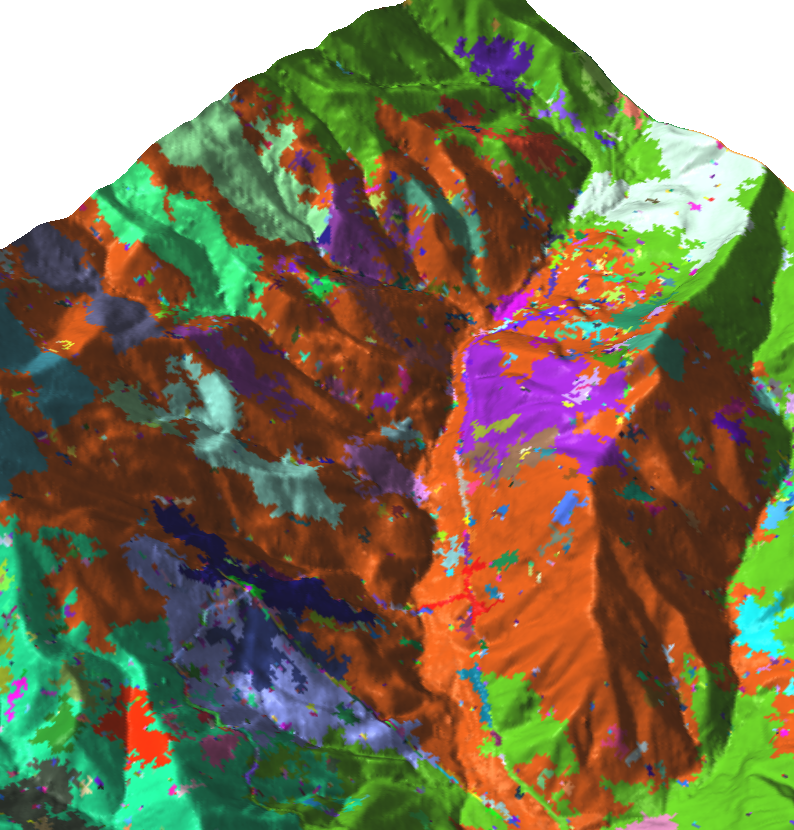
\includegraphics[width=\textwidth]{grass/segment_on_counts}
\end{center}

% method=n class=2
% method=n class=1
% i.group
% i.segement 0.75

\end{column}
\end{columns}

\end{frame}

%%%%%%%%%%%%%%%%%%%%%%%%%%%%%%%%%%%%%%%%%%%%%%%%%%%%%%%%%%%%%%%%%%%%%
\begin{frame}{r.in.lidar: compute height above a given raster during binning}

\gmodule{r.in.lidar} -- compute height above given surface (\texttt{base\_raster})

\begin{center}
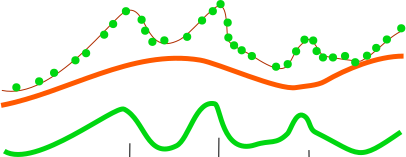
\includegraphics[height=0.5\textheight]{images/features/base_raster}
\end{center}

The resolutions of binning and ground raster can differ.

\end{frame}

% r.in.lidar output=height_max_10m method=max base_raster=ground_mean_neighbors resolution=10 class_filter=1
% 522,357,379 points from 90 files
% 48 MB
% 4 min 30 sec

%%%%%%%%%%%%%%%%%%%%%%%%%%%%%%%%%%%%%%%%%%%%%%%%%%%%%%%%%%%%%%%%%%%%%
\begin{frame}{r.in.lidar: \texttt{base\_raster} workflow}

\begin{columns}
\begin{column}{0.45\textwidth}

\texttt{r.in.lidar method=mean class=2}\\
\ $\square\hspace{-4pt}\leftarrow$ 29 million points from 90 files\\
\ $\square\hspace{-4pt}\rightarrow$ ground with NULLs (8$\times$8km, 1m)\\
%\ $\cdot$ in 2 min using 480MiB
% \ $\cdot$ 8076 $\times$ 7223 = 58,332,948 (1m)

\texttt{r.neighbors size=25}\\
\ $\square\hspace{-4pt}\leftarrow$ ground with NULLs\\
\ $\square\hspace{-4pt}\rightarrow$ continuous ground\\
%\ $\cdot$ in 2.5 min\\
% \ $\cdot$ 8076 $\times$ 7223 = 58,332,948 (1m)

\texttt{r.in.lidar method=max\\\ resolution=10 class\_filter=1}\\
\ $\square\hspace{-4pt}\leftarrow$ 522 million points from 90 files\\
\ $\square\hspace{-4pt}\leftarrow$ continuous ground\\
\ $\square\hspace{-4pt}\rightarrow$ max veg height per 10m cell\\
%\ $\cdot$ in 4.5 min using 48 MiB

\medskip
\footnotesize
9 min, 480 MiB, Ubuntu, 2.7 GHz, SSD
% (R 2150MB/s, W 1200MB/s)
\\
578 million points in 90 files

\end{column}
\begin{column}{0.45\textwidth}

\begin{center}
  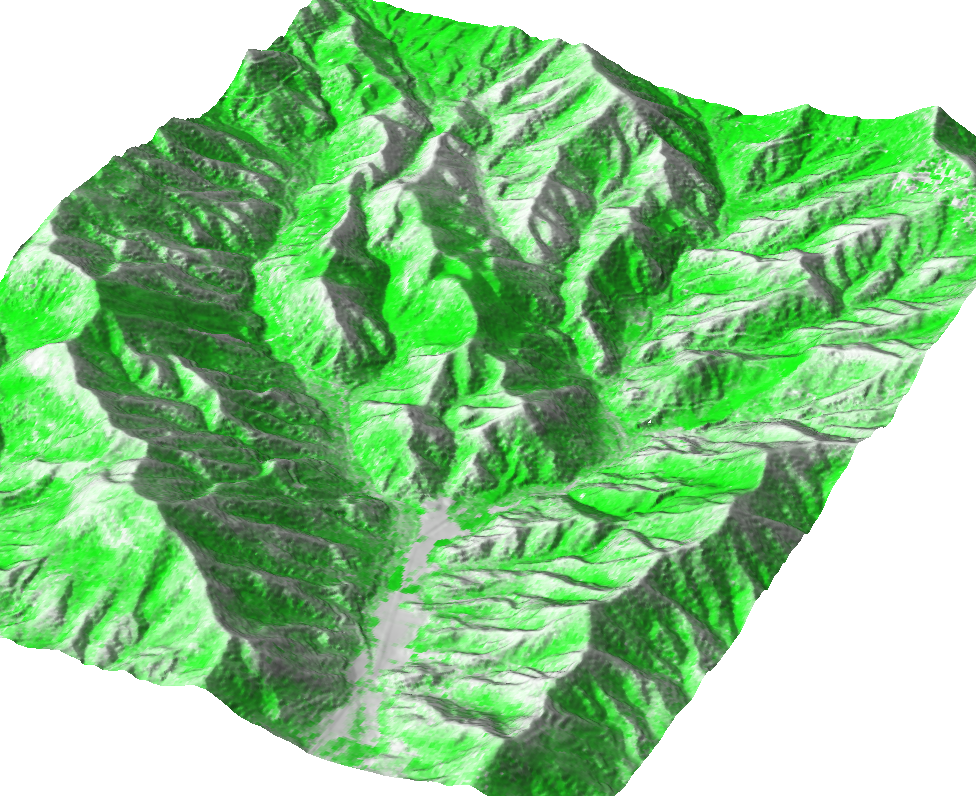
\includegraphics[width=\textwidth]{grass/max_height_10m_on_ground_from_neighbors_smaller_area_top}
\end{center}

\end{column}
\end{columns}

\end{frame}


%%%%%%%%%%%%%%%%%%%%%%%%%%%%%%%%%%%%%%%%%%%%%%%%%%%%%%%%%%%%%%%%%%%%%
\begin{frame}{r3.in.lidar}

\begin{columns}
\begin{column}{0.28\textwidth}

\begin{itemize}
  \item generally similar to \gmodule{r.in.lidar}
  \item 3D raster
  \item proportional count
  \begin{itemize}
    \item count per 3D cell relative to the count per vertical column
  \end{itemize}
  \item intensity can be used instead of count
\end{itemize}

\bigskip
\footnotesize
under development

\end{column}
\begin{column}{0.7\textwidth}

\begin{center}
  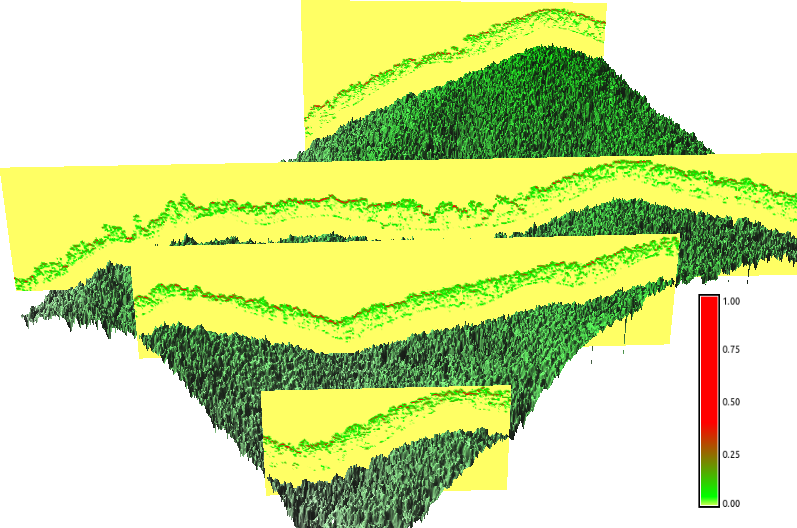
\includegraphics[width=\textwidth]{grass/red_green_3d}
\end{center}

\end{column}
\end{columns}

\end{frame}

% vis also possible using Tangible Landscape

%%%%%%%%%%%%%%%%%%%%%%%%%%%%%%%%%%%%%%%%%%%%%%%%%%%%%%%%%%%%%%%%%%%%%
\begin{frame}{v.in.lidar}

\begin{columns}
\begin{column}{0.28\textwidth}

\begin{itemize}
  \item filtering same as in \gmodule{r.in.lidar}
  \item 3D vector
  \item used together with
  \begin{itemize}
    \item \gmodule{r.in.lidar}
    \item interpolation modules (\gmodule{v.surf.rst}, \gmodule{v.surf.bspline}, \gmodule{v.surf.idw})
  \end{itemize}
  \item decimation
  \item polygons as a mask
\end{itemize}

\end{column}
\begin{column}{0.7\textwidth}

\begin{center}
  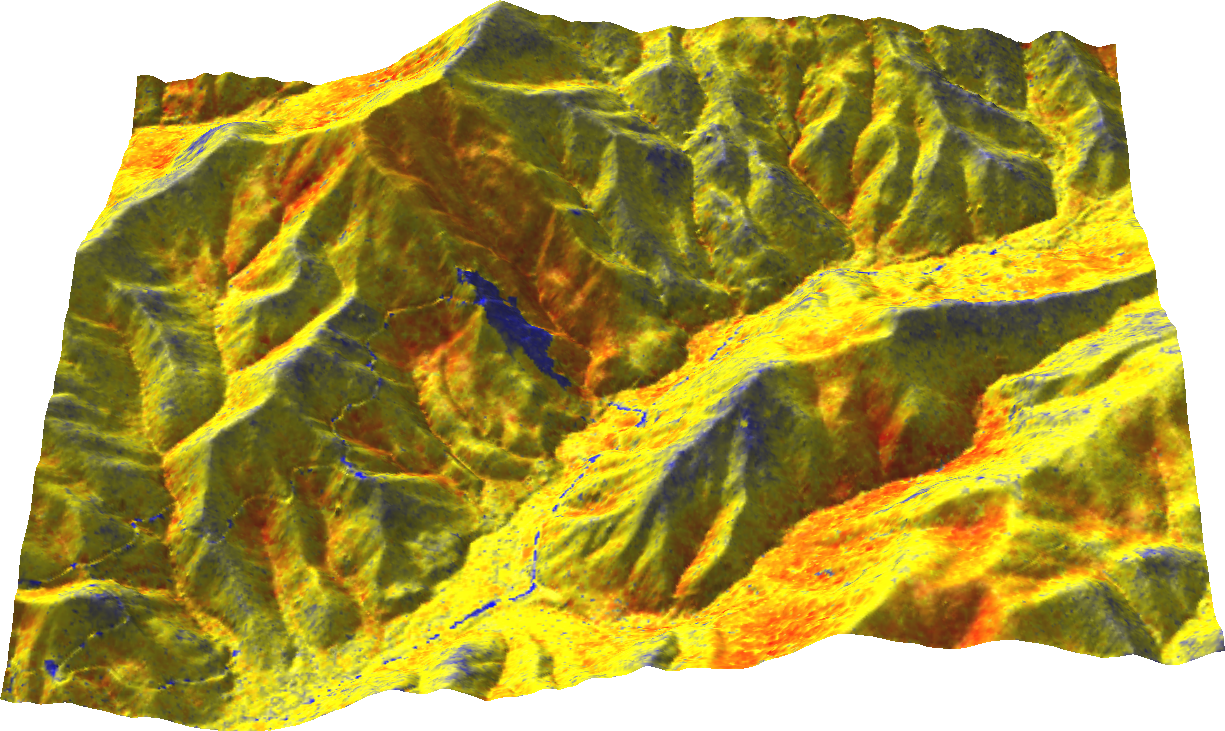
\includegraphics[width=\textwidth]{grass/range_on_ground_from_north}

  \footnotesize
  range from \gmodule{r.in.lidar} on ground obtained
  from \gmodule{v.in.lidar} followed by \gmodule{v.surf.rst}
\end{center}

\end{column}
\end{columns}

\end{frame}


%%%%%%%%%%%%%%%%%%%%%%%%%%%%%%%%%%%%%%%%%%%%%%%%%%%%%%%%%%%%%%%%%%%%%
\begin{frame}{Comparison of count-based and grid-based decimation}

\begin{center}
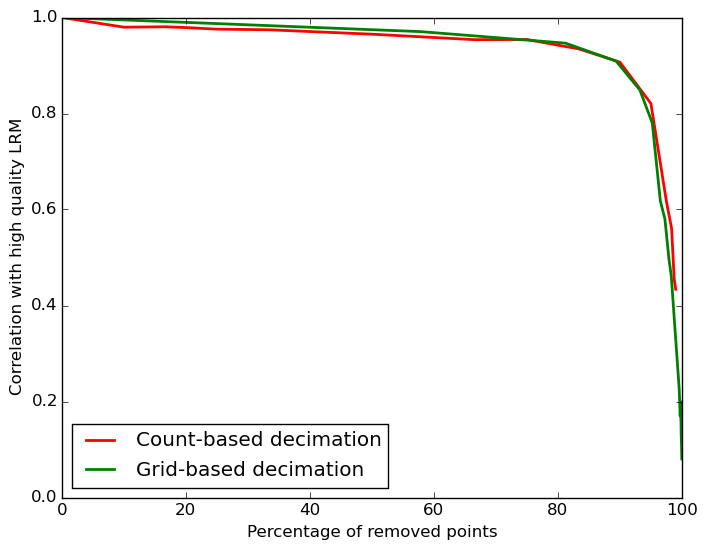
\includegraphics[height=0.8\textheight]{lrm_comparison_grid_count}
\end{center}

\end{frame}


%%%%%%%%%%%%%%%%%%%%%%%%%%%%%%%%%%%%%%%%%%%%%%%%%%%%%%%%%%%%%%%%%%%%%
\begin{frame}{Crop the point cloud by polygon}

\gmodule{v.in.lidar} -- limit the import to selected areas (2D)

\bigskip
\bigskip

\centering
\begin{minipage}{0.96\textwidth}
\centering
%
\newcommand{\imgsize}{0.23\textwidth}

\includegraphics[width=\imgsize]{features/areas}%
~%
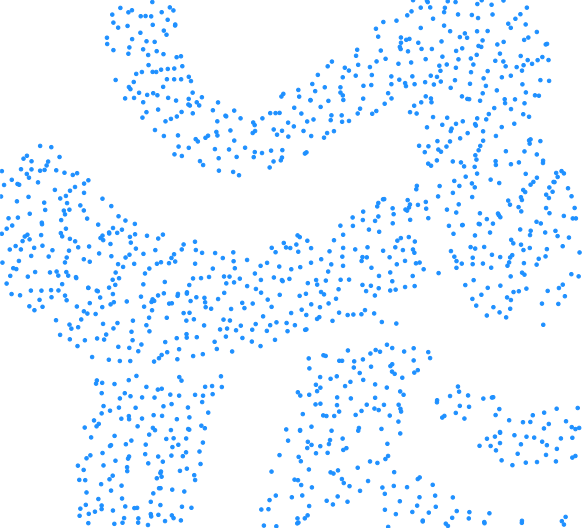
\includegraphics[width=\imgsize]{features/selected_1}%
~%
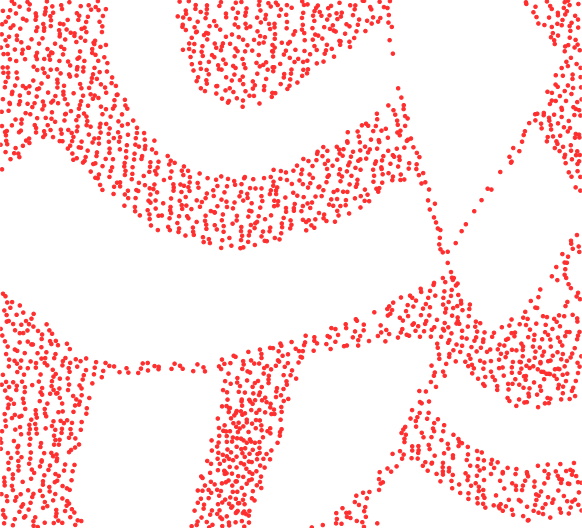
\includegraphics[width=\imgsize]{features/selected_2}%

\newcommand{\captionfont}{\scriptsize\tt}%
% using phantom to vertically stretch to have space for p
\makebox[\imgsize][c]{\captionfont areas\vphantom{patch}}%
~%
\makebox[\imgsize][c]{\captionfont v.in.lidar mask=}%
~%
\makebox[\imgsize][c]{\captionfont v.in.lidar -i mask=}%
%
\end{minipage}

\end{frame}


%%%%%%%%%%%%%%%%%%%%%%%%%%%%%%%%%%%%%%%%%%%%%%%%%%%%%%%%%%%%%%%%%%%%%
\begin{frame}{Speed optimization}

\begin{block}{\gmodule{r.in.lidar}}
 \begin{itemize}
  \item choose computation region extent and resolution ahead
  \item have enough memory to avoid using \texttt{percent} option
 \end{itemize}
\end{block}


\begin{block}{\gmodule{v.in.lidar}}
 \begin{itemize}
  \item \texttt{-r} limit import to computation region extent
  \item \texttt{-t} do not create attribute table
  \item \texttt{-b} do not build topology (applicable to other modules as well)
  \item \texttt{-c} store only coordinates, no categories or IDs
 \end{itemize}
\end{block}

\end{frame}

%%%%%%%%%%%%%%%%%%%%%%%%%%%%%%%%%%%%%%%%%%%%%%%%%%%%%%%%%%%%%%%%%%%%%
\begin{frame}{Memory requirements}

\begin{block}{\gmodule{r.in.lidar}}
 \begin{itemize}
  \item depend on the side of output and type of analysis
  \item can be reduced by \texttt{percent} option
  \item \texttt{ERROR: G\_malloc: unable to allocate ... bytes of memory}
  \item on Linux available memory for process is RAM + SWAP partition
 \end{itemize}
\end{block}


\begin{block}{\gmodule{v.in.lidar}}
 \begin{itemize}
  \item low when not building topology
  \item \texttt{export GRASS\_VECTOR\_LOWMEM=1}
 \end{itemize}
\end{block}

\end{frame}

%%%%%%%%%%%%%%%%%%%%%%%%%%%%%%%%%%%%%%%%%%%%%%%%%%%%%%%%%%%%%%%%%%%%%
\begin{frame}{Limits}

\begin{itemize}
  \item vector features with topology:
    count limit is about 2 billion features per vector map
    % 2 $\hat{}$ 31 - 1
  \item points without topology:
    count theoretically limited only by the 64bit architecture\\
    (may be 16~exbibytes per file but depends on the file system)
  % \item for large vectors with attributes PostgreSQL backend is recommended
  \item more limits for 32bit versions for operations which require memory
    % watersheds, half basins, flow accumulation, drainage directions, and stream
%  \item read/write to disk often limits speed (faster for rasters in 7.1)
  \item number of open files limitation (system limit)
  \begin{itemize}
   \item often 1024, change using \emph{ulimit} on Linux
  \end{itemize}
  \item \gmodule{r.watershed} 90,000 x 100,000 (9 billion cells) in 77.2 hours (2.93GHz)
  \item
    \gmodule{v.surf.rst}: minutes = 1.5e-11 * points$^2$
    {\footnotesize (test: 13 min for 1 million points and 201880 cells)}
  \item read the documentation
  \item write to \href{https://lists.osgeo.org/listinfo/grass-user}{grass-user mailing list}
    or \href{http://trac.osgeo.org/grass/}{GRASS GIS Tracker} in case you hit limits
\end{itemize}

\end{frame}


%%%%%%%%%%%%%%%%%%%%%%%%%%%%%%%%%%%%%%%%%%%%%%%%%%%%%%%%%%%%%%%%%%%%
\begin{frame}{v.out.lidar}

\begin{columns}
\begin{column}{0.28\textwidth}

exports points in a vector map as lidar points

\begin{itemize}
\item visualization (plas.io, CloudCompare)
\item further processing (PDAL, libLAS, CloudCompare, \ldots)
\item testing workflows with generated data
\end{itemize}

\end{column}
\begin{column}{0.7\textwidth}

\begin{center}
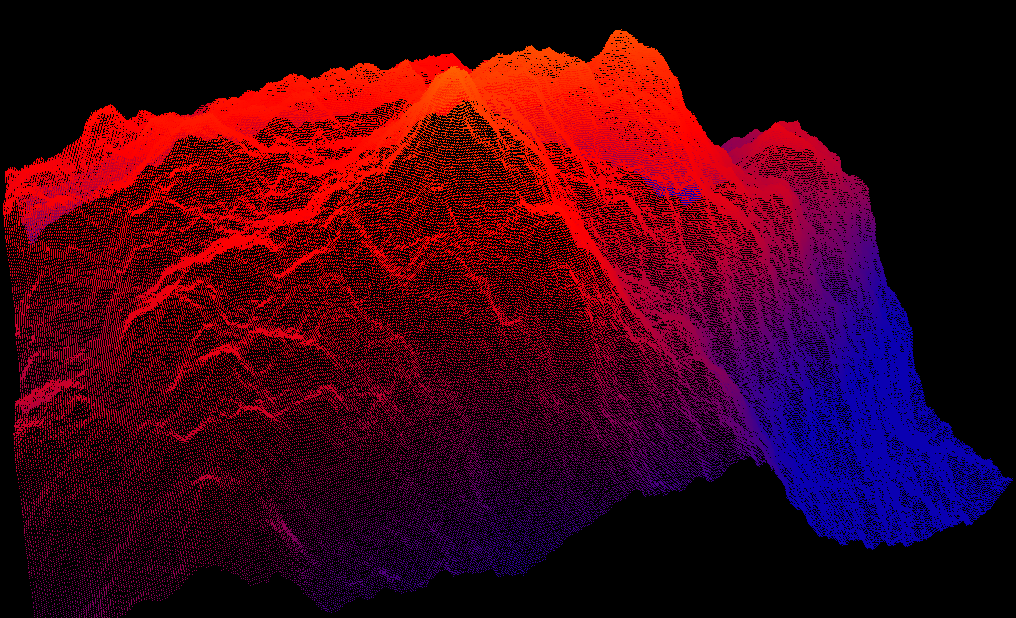
\includegraphics[height=0.5\textheight]{images/features/fractals_plasio}

\gmodule{r.surf.fractal} output in \href{http://plas.io}{plas.io}
\end{center}

% g.region rows=1669 cols=2515 cells=4197535
% r.surf.fractal out=test
% r.to.vect -z t=p in=test out=test -b
% v.out.lidar in=test out=test.las

\end{column}
\end{columns}

\bigskip

More smaller tools under development.

\end{frame}


%%%%%%%%%%%%%%%%%%%%%%%%%%%%%%%%%%%%%%%%%%%%%%%%%%%%%%%%%%%%%%%%%%%%%
\begin{frame}{v.lidar.edgedetection suite}

\begin{columns}
\begin{column}{0.28\textwidth}

\begin{itemize}
  \item \gmodule{v.lidar.edgedetection}
  \item \gmodule{v.lidar.growing}
  \item \gmodule{v.lidar.correction}
  \item uses return information
\end{itemize}

\end{column}
\begin{column}{0.7\textwidth}

\begin{center}
  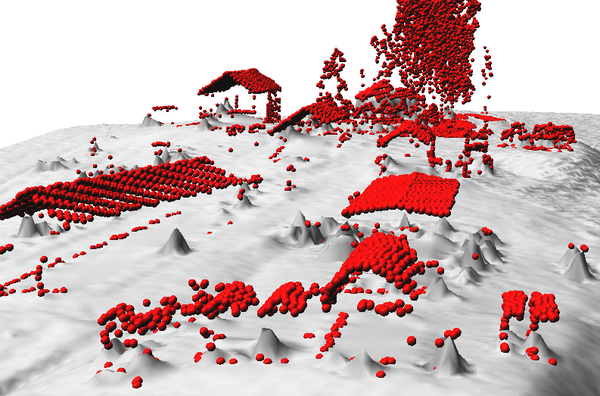
\includegraphics[width=\textwidth]{grass/v_lidar_edgedetection_objects}
\end{center}

\end{column}
\end{columns}

\end{frame}


%%%%%%%%%%%%%%%%%%%%%%%%%%%%%%%%%%%%%%%%%%%%%%%%%%%%%%%%%%%%%%%%%%%%%
\begin{frame}{v.lidar.mcc}

\begin{columns}
\begin{column}{0.28\textwidth}

\begin{itemize}
  \item ground and non-ground
  \item multiscale curvature based classification algorithm
\end{itemize}

\end{column}
\begin{column}{0.7\textwidth}

\begin{center}
  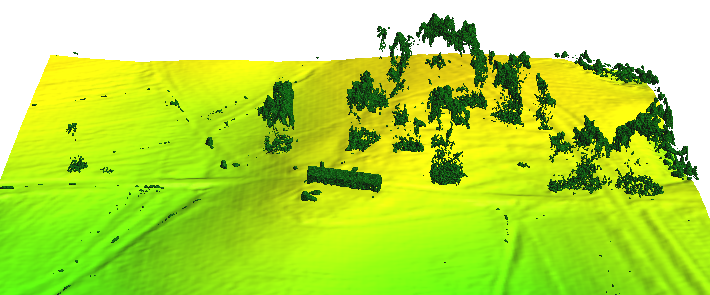
\includegraphics[width=\textwidth]{grass/mcc_default}
\end{center}

\end{column}
\end{columns}

\end{frame}


%%%%%%%%%%%%%%%%%%%%%%%%%%%%%%%%%%%%%%%%%%%%%%%%%%%%%%%%%%%%%%%%%%%%%
\begin{frame}{r.skyview}

\begin{itemize}
  \item sky-view factor
\end{itemize}

\begin{center}
  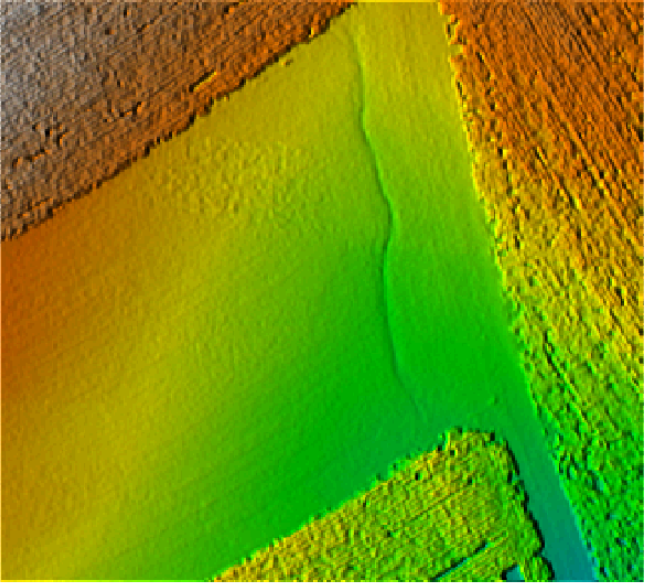
\includegraphics[width=0.4\textwidth]{vis/shaded_relief}
  ~~
  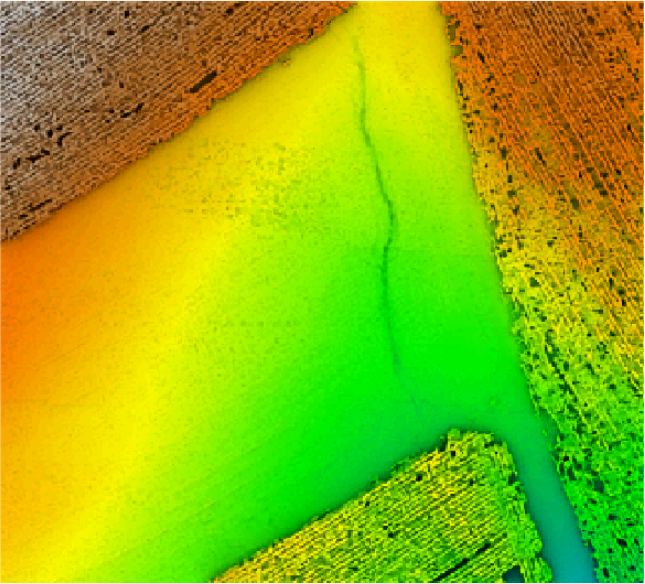
\includegraphics[width=0.4\textwidth]{vis/skyview}
\end{center}

\end{frame}


%%%%%%%%%%%%%%%%%%%%%%%%%%%%%%%%%%%%%%%%%%%%%%%%%%%%%%%%%%%%%%%%%%%%%
\begin{frame}{r.local.relief}

\begin{itemize}
  \item local relief model
\end{itemize}

\begin{center}
  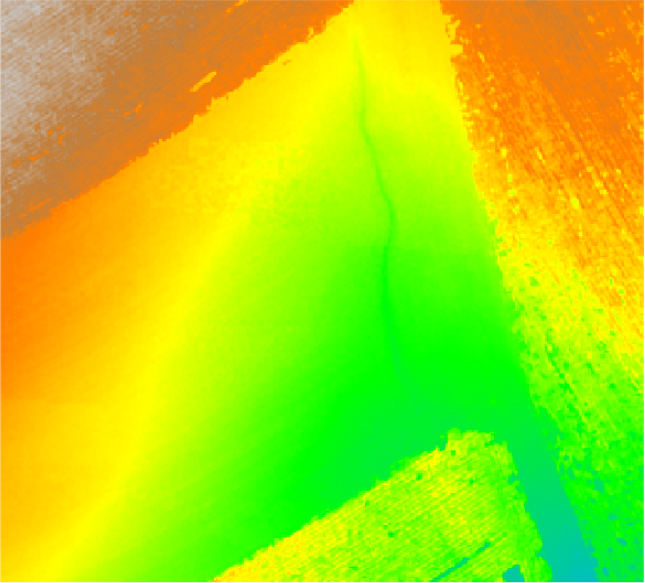
\includegraphics[width=0.4\textwidth]{vis/elevation}
  ~~
  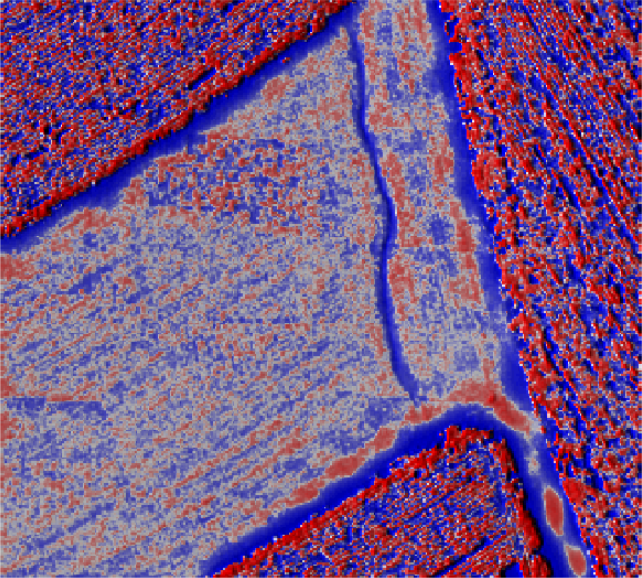
\includegraphics[width=0.4\textwidth]{vis/lrm}
\end{center}

\end{frame}


%%%%%%%%%%%%%%%%%%%%%%%%%%%%%%%%%%%%%%%%%%%%%%%%%%%%%%%%%%%%%%%%%%%%%
\begin{frame}{r.shaded.pca}

\begin{columns}
\begin{column}{0.35\textwidth}

\begin{itemize}
  \item relief shades from various directions
  \item combined into RGB composition
\end{itemize}

\end{column}
\begin{column}{0.6\textwidth}

\begin{center}
  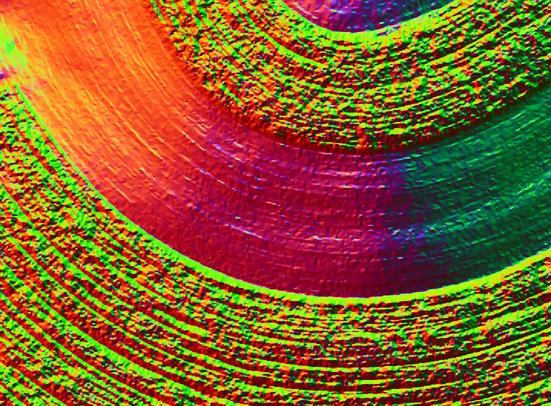
\includegraphics[width=\textwidth]{grass/agisoft_shadedpca100}
\end{center}

\end{column}
\end{columns}

\end{frame}


%%%%%%%%%%%%%%%%%%%%%%%%%%%%%%%%%%%%%%%%%%%%%%%%%%%%%%%%%%%%%%%%%%%%%
\begin{frame}{Integration with PDAL}

\begin{block}{experimental}
 \begin{itemize}
  \item \module{v.in.pdal}
  \item reprojection during import
  \item ground filter
    (alternative to \gmodule{v.lidar.edgedetection} or \gmodule{v.lidar.mcc})
  \item compute height as a difference from ground
 \end{itemize}
\end{block}

\begin{block}{planned}
 \begin{itemize}
  \item \module{r.in.pdal}, \module{r3.in.pdal}, \module{v.out.pdal}, \module{r.out.pdal}, \ldots
  \item more PDAL filters
 \end{itemize}
\end{block}

\end{frame}


%%%%%%%%%%%%%%%%%%%%%%%%%%%%%%%%%%%%%%%%%%%%%%%%%%%%%%%%%%%%%%%%%%%%%
\begin{frame}{GRASS GIS lidar tools roadmap}

 \begin{itemize}
  \item now: basic tools available in GRASS GIS 7.0
    \begin{itemize}
      \item \href{https://grass.osgeo.org/news/54/15/GRASS-GIS-7-0-3-released/}{7.0.3 released this January}
        with 64bit support for MS Windows
    \end{itemize}
  \item now: presented functionality available for testing in development version of GRASS GIS
    \begin{itemize}
      \item daily build for MS Windows and Ubuntu
      \item self-compiled version (simple for Fedora, CentOS, \ldots\ possible on Mac OS)
    \end{itemize}
  \item summer: 3D raster, PDAL, 2D display, smooth reprojections
  % color support, standardized categories
  \item fall/winter: backport of stable functionality to 7.0 or release of 7.1
  % 3D display, direct interpolation, direct processing
 \end{itemize}

\end{frame}


%%%%%%%%%%%%%%%%%%%%%%%%%%%%%%%%%%%%%%%%%%%%%%%%%%%%%%%%%%%%%%%%%%%%%
\begin{frame}{Acknowledgements}

% logo at the bottom can be moved down
\vspace*{0.05\textheight}

\begin{block}{Software: GRASS GIS}
Presented functionality are work done by Vaclav Petras, Markus Metz, and the GRASS development team.
Thanks to users for feedback and testing, especially to Doug Newcomb, Markus Neteler, and William Hargrove.
\end{block}

\begin{block}{Dataset: Nantahala NF, NC: Forest Leaf Structure, Terrain and Hydrophysiology}
Lidar data acquisition and processing completed
by the National Center for Airborne Laser Mapping (\href{http://www.ncalm.org}{NCALM}).
NCALM funding provided by NSF's Division of Earth Sciences, Instrumentation and Facilities Program.
EAR-1043051. \url{http://dx.doi.org/10.5069/G9HT2M76}
\end{block}

\end{frame}


%%%%%%%%%%%%%%%%%%%%%%%%%%%%%%%%%%%%%%%%%%%%%%%%%%%%%%%%%%%%%%%%%%%%%
\begin{frame}{}

% logo at the bottom can be moved down
\vspace*{0.05\textheight}

\begin{block}{Summary}
 \begin{itemize}
  \item rasterize early
  \item make use of existing methods for raster and vector processing
  \item 3D rasters, PDAL integration
  \item the plan for next 30 years driven by users
    -- \href{https://lists.osgeo.org/listinfo/grass-user}{grass-user mailing list}
 \end{itemize}
\end{block}

\bigskip

\centering
\href{https://grass.osgeo.org/download/}{%
Get GRASS GIS 7.1 development version at\\
\texttt{grass.osgeo.org/download}%
}

\smallskip


\includegraphics[height=0.25\textheight]{logos/grass_gis}

% this is for logo without text
%\vspace*{-1.5ex}
%\Large
%\textbf{GRASS} GIS

\end{frame}


\end{document}
